\documentclass[12pt]{book}
\usepackage[utf8]{inputenc}
\usepackage[margin=1.25in]{geometry}
\usepackage{graphicx}
\usepackage{amsmath , amssymb}
\usepackage{bm}
\usepackage{esvect}
\usepackage{centernot}
\newcommand{\lagrange}{\mathcal{L}}
\newcommand{\fourier}{\mathcal{F}}


\begin{document}
    \chapter{Transformation de laplace}
        \section{Definition}
            La transformation de laplace est une technique mathematique utilise pour transferer une fonction $f(t)$ du domain temporel au domain frequenciel complex $F(s)$
            \\ $f(t) \implies F(s)$ ,$t$ en seconds $(s)$ , s en radiant par second $(rd/s)$ , $s=a+ib$ \\
            \begin{center}
                \boxed{F(s) = \lagrange \{ f(t) \}= \int^\infty_0f(t)e^{-st}dt }
            \end{center}
        \section{Fonction unite $u(t)$}
            \begin{center}
                \begin{minipage}{0.49\linewidth}
                    $u(t) = 
                    \begin{cases}
                        1, & t \geq 0 \\
                        0, & t < 0
                      \end{cases}
                      $
                \end{minipage}
                \begin{minipage}{0.39\linewidth}
                    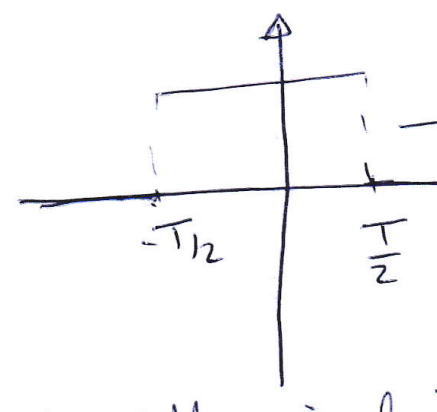
\includegraphics[width = \linewidth]{pic/fonctionunite.png}
                \end{minipage}
            \end{center}
            \underline{propriete} \\ 
            \begin{itemize}
                \item pour une fonction $f(t)$ soit transformer en domain complex elle va etre une multiple de $u(t)$
                    \begin{center}
                        $f(t)u(t) = \begin{cases}
                            f(t) & t \geq 0 \\
                            0 & t< 0
                        \end{cases}$
                    \end{center}
                \item  si $u(t)$ est multiplie par une constante $k \implies ku(t) \begin{cases}
                    k & t \geq 0 \\
                    0 & t < 0
                \end{cases}$
                \item Decalage en temp 
                    \begin{itemize}
                        \item decalage vers la droite 
                        \begin{center}
                            \begin{minipage}{0.49\linewidth}
                                $ku(t-a) = 
                                \begin{cases}
                                    k, & t \geq a \\
                                    0, & t < a
                                \end{cases}
                                $
                            \end{minipage}
                            \begin{minipage}{0.39\linewidth}
                                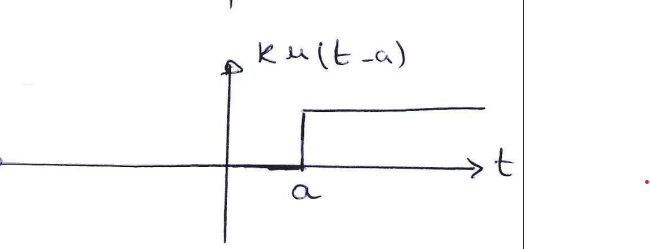
\includegraphics[width = \linewidth]{pic/droitdecalageunite.png}
                            \end{minipage}
                        \end{center}
                        \item decalage vers la gauche 
                        \begin{center}
                            \begin{minipage}{0.49\linewidth}
                                $ku(t+a) = 
                                \begin{cases}
                                    k, & t \geq -a \\
                                    0, & t < -a
                                \end{cases}
                                $
                            \end{minipage}
                            \begin{minipage}{0.39\linewidth}
                                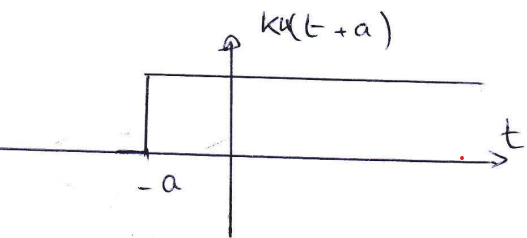
\includegraphics[width = \linewidth]{pic/gauchedecalageunite.png}
                            \end{minipage}
                        \end{center}
                    \end{itemize}
            \end{itemize}
        \section{fonction implusion (delta de dirac) $\delta(t)$}
            \begin{center}
                \begin{minipage}{0.49\linewidth}
                    $  
                    \begin{cases}
                        \delta(t) =0 , & t \not = 0 \\
                        \int^\infty_{-\infty}\delta(t)dt =1, & t =0
                    \end{cases}
                    $
                \end{minipage}
                \begin{minipage}{0.39\linewidth}
                    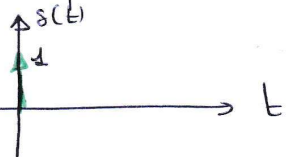
\includegraphics[width = \linewidth]{pic/deltadirac.png}
                \end{minipage}
            \end{center}
            \underline{propriete}
            \begin{itemize}
                \item multiplication par une constante k
                    \begin{center}
                        \begin{minipage}{0.49\linewidth}
                            $  
                            \begin{cases}
                                k\delta(t) =0 , & t \not = 0 \\
                                \int^\infty_{-\infty}k\delta(t)dt =k, & t =0
                            \end{cases}
                            $
                        \end{minipage}
                        \begin{minipage}{0.39\linewidth}
                            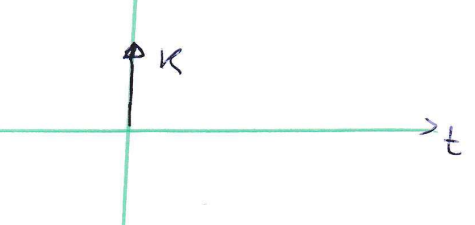
\includegraphics[width = \linewidth]{pic/kdeltadirac.png}
                        \end{minipage}
                    \end{center}
                \item decalage 
                    \begin{center}
                        \begin{minipage}{0.49\linewidth}
                            $  
                            \begin{cases}
                                k\delta(t-a) =0 , & t \not = a \\
                                \int^\infty_{-\infty}k\delta(t -a)dt =k, & t =a
                            \end{cases}
                            $
                        \end{minipage}
                        \begin{minipage}{0.39\linewidth}
                            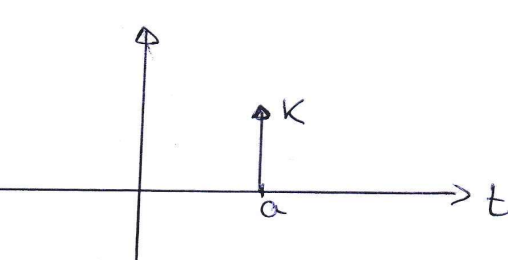
\includegraphics[width = \linewidth]{pic/decalagedirac.png}
                        \end{minipage}
                    \end{center}
                \item $\int^\infty_{-\infty}f(t)\delta(t-a) = \int^\infty_{-\infty}f(a)\delta(t-a)=f(a)$ car $f(t)\delta(t-a)$ \\ pour tout $t \not = a$ est 0
                \item $\delta(\alpha t) = \frac{1}{|\alpha|}\delta(t)$
                \item $\delta(t) = \delta(-t)$ (fonction pair)
                \item $\delta(t) = \frac{du(t)}{dt}$
            \end{itemize}
        \section{Propriete de la transformation de lapalce}
            \begin{itemize}
                \item Leniarite $af(t) +bf(t)\overset{\lagrange}{\rightleftarrows} aF(s) + bG(s) $
                \item Decalage dans le domain frequenciel $e^{-at}f(t)u(t)\overset{\lagrange}{\rightleftarrows}F(s+a)$
                \item Decalage dans le domain temps $f(t-a)u(t-a)\overset{\lagrange}{\rightleftarrows}e^{-as}F(s)$
                \item Differentielle \\
                    $ \lagrange \{ f^{'}(t)\}= sF(s) - f(0)  $ \\
                    $ \lagrange \{ f^{''}(t)\} = s^2F(s) - sf(0) - f^{'}(0)  $ \\
                    $\lagrange\{ f^n(t) \} = s^nF(s) - s^{n-1}f(0)-s^{n-2}f^{'}(0)\ldots sf^{n-2}(0)-f^{n-1}(0)$
                \item Integration \
                    $ \lagrange \{ \int^t_0f(x)dx \} = \frac{F(s)}{s} $
                \item  Multiplication par t 
                    $f(t) \overset{\lagrange}{\rightleftarrows} F(s) \implies \lagrange\{ tf(t) \}=\frac{-dF(s)}{ds} $  
                \item Theorem de valeur initiale $f(0) = \lim_{s\to\infty}sF(s)$
                \item theorem de valeur finale $\lim_{t\to\infty}f(t)=\lim_{x\to 0}sF(s)$
                \item Transformation temporelle $f(at-b)u(at-b)\overset{\lagrange}{\rightleftarrows}\frac{e^{-s\frac{b}{a}}}{a}F(\frac{s}{a})$
                \item Theoreme de convolution \\
                    la convolution de 2 fonction $x(t)$ et $h(t)$ est \\
                    $y(t)= x(t)*h(t) = \int_{-\infty}^{+\infty}x(\varphi)h(t-\varphi)d\varphi$ \\
                    $Y(s) = \lagrange\{ x(t) * h(t) \} = X(s).H(s)$
            \end{itemize}
        \pagebreak
        \section{Transformation de laplace inverse}
            \subsection{Methode de decomposition }
            on a : $F(p) = \frac{N(p)}{D(p)}$ 
                \begin{itemize}
                    \item chaque valeur de (p) qui anule le numerateur est apple un pole
                    \item chaque valeur de (p) qui anulle le denominateur est apple un pole 
                \end{itemize}
            \underline{Cas 1 } : tout les poles sont des racine simple (distinctes) \\
            $$ F(p) = \frac{N(p)}{(p-p_1)(p-p_2)(p-p_3)\ldots(p-p_k) \ldots(p-p_n)} $$ avec $p_1 \not = p_2 \not = p_3 \not = p_k  \ldots \not = p_n$ \\
            dans ce cas la forme decompose de $F(p)$ sera :\\
            $$  F(p) = \frac{A_1}{(p-p_1)}+\frac{A_2}{(p-p_2)}+\frac{A_3}{(p-p_3)}+\ldots+\frac{A_k}{(p-p_k)}+\ldots+\frac{A_n}{(p-p_n)} $$
            avec $A_k = \lim_{p\to p_k}(p-p_k)F(p)$ \\
            \underline{Cas 2} : il existe un pole $p_k$ qui une racine de multiplicite m \\
            $$ F(p) = \frac{N(p)}{\ldots (p-p_k)^m \ldots} $$
            dans ce cas la forme decompose de $F(p)$ sera 
            $$ F(p) = \ldots + \frac{A_1}{(p-p_k)} + \frac{A_2}{(p-p_k)^2} + \ldots +\frac{A_i}{(p-p_k)^i} + \ldots \frac{A_m}{(p-p_k)^m} +\ldots $$
            avec $A_i = \frac{1}{(m-i)!}\lim_{p\to p_k}\frac{d^{m-i}}{dp^{m-i}} \left[ (p-p_k)^mF(p) \right] $
            \\ \underline{Note } dans le cas ou la degre de $N(p) >$ degre de $D(p)$ en peut ecrire $F(p)$ sous la form $\underbrace{X(p)}_{entier} + \frac{N^{'}(p)}{D(p)}$ ou $N^{'}(p) < D(p)$
        \pagebreak
        \section{Tableau de transformation} 
        
            \begin{table}[h]
                \LARGE
                \centering
                \begin{tabular}{|c|c|}
                    \hline
                    $ f(t) $ & $\lagrange(f)$ \\ \hline
                    $ t^n_{n=1,2,\ldots} $ & $\frac{n!}{s^{n+1}}$  \\ \hline
                    $ t^a_{a>0} $ & $\frac{T(a+1)}{s^{a+1}}$ \\ \hline
                    $ e^{at} $ & $\frac{1}{s-a}$ \\ \hline
                    $ \cos(wt) $ & $\frac{s}{s^2 + w^2}$ \\ \hline
                    $ \sin(wt) $ & $\frac{w}{s^2+w^2}$ \\ \hline
                    $\cosh(at)$ & $\frac{s}{s^2-a^2}$  \\ \hline
                    $ \sinh(at) $ & $ \frac{a}{s^2-a^2} $ \\ \hline
                \end{tabular}
            \end{table}
        \section{Application }
            \subsection{Equation differentiell ordinair avec condition initial}
                \subsubsection*{Equation 1 }
                    $$ \frac{2dy}{dt} +5y = e^{-2t}u(t) \;,\; y(0) = 2 $$
                    $\lagrange\{ \frac{2dy}{dt}+5y \} = \lagrange\{ e^{-2t}u(t) \}$\\ 
                    $\implies \lagrange\{ \frac{2dy}{dt}\}+ \lagrange\{5y \} = \lagrange\{ e^{-2t}u(t) \}$ (lineairite) \\
                    $2[sY-y(0)]+5Y = \frac{1}{s+2} \implies Y =\frac{4s +9}{(s+2)(2s+5)}=\frac{2s + \frac{9}{2}}{(s+2)(s+\frac{5}{2})}$ \\
                    en peut decomposer $Y$ sous la form $ Y=\frac{A}{(s+2)} + \frac{B}{s+\frac{5}{2}} $ \\
                    avec \begin{itemize}
                        \item $A = \lim_{s\to -2}(s+2)Y=\frac{-4 + \frac{9}{2}}{-2 + \frac{5}{2}}=1$
                        \item $B = \lim_{s\to \frac{-5}{2}} (s+\frac{5}{2})Y = \frac{-5 + \frac{9}{2}}{\frac{-5}{2}+2} = 1$
                    \end{itemize}
                    $Y = \frac{1}{s+2}+\frac{1}{s+\frac{5}{2}} \implies$\boxed{y = (e^{-2t}+e^{-\frac{5}{2}t} )u(t)}
                \subsubsection*{Equation 2}
                $$ y^{''}(t) +3y^{'}+2y(t) = e^{-t}u(t) \; , \; y(0) = y^{'}(0)=0 $$
                appliquee laplace $\implies s^2Y+sy(0)-y^{'} +3y(0) + 2Y = \frac{1}{s+1} $\\
                $\implies Y - \frac{1}{(s+1)(s^2+3s+3)}=\frac{1}{(s+1)^2(s+2)}$ \\
                en peut decompose $Y$ sous la form : $Y = \frac{A}{(s+2)}+\frac{B}{(s+1)^2}+\frac{C}{s+1}$
                \begin{itemize}
                    \item $A = \lim_{s \to -2}(s+2)Y = \frac{1}{(s+2+1)^2}=1$
                    \item $B = \lim_{s \to -1}(s+1)Y =1$
                    \item $V = \lim_{s \to -1}\frac{d}{ds}(s+1)^2Y = \lim_{s \to -1} \frac{d}{ds}\frac{1}{s+2} = \lim_{s \to -1}\frac{-1}{(s+2)^2} = -1$
                \end{itemize}
                $Y = \frac{1}{s+2}+\frac{1}{(s+1)^2}-\frac{1}{s+1} \implies y = (e^{-2t}+te^{-t}-e^{-t})u(t)$
            \subsection{Mecanique (oscillateur harmonique simple)}
                Une mass $(m)$ conecte a un ressort de constant $(k)$ ,$x$ est la distance que le ressort est tire de sa position d'equilibre \\
                L equation de mouvement est :\begin{center}
                    $\frac{d^2x}{dt^2}+\frac{k}{m}x = 0$ 
                \end{center}
                Dans le cas d amortissement , une force de frottement $\vv{f} = -b\vv{v}$ avec $b$ est la coefficient d amortisment , lequation de mouvement est :
                \begin{center}
                    $\frac{d^2x}{dt^2}+\frac{b}{m}\frac{dx}{dt}+\frac{k}{m}x = 0 $\\ $b =2\delta\sqrt{mk} \; , \; \delta $ est le rapport d amortissement
                \end{center}
                Dans le cas ou loscillateu harmonique est soumis a une force exterieur $F(t)$ l equation devient 
                $$ \frac{d^2x}{dt^2}+2\delta w_0 \frac{dx}{dt} + w_0^2x = \frac{F(t)}{m} $$ avec $w_0^2 =\frac{k}{m}$
                \pagebreak
            \subsection{Systeme lineaire invariant avex le temp (LTI)}
               \begin{center}
                    \begin{minipage}{0.49\linewidth}
                        Considerons un systeme (LTI) caracterise par :
                        \begin{itemize}
                            \item $x(t) $ : fonction d entre 
                            \item $h(t) $ : impulsion reponse 
                            \item $y(t) $ : fonction de sortie
                        \end{itemize}
                    \end{minipage}
                    \begin{minipage}{0.49\linewidth}
                        
                        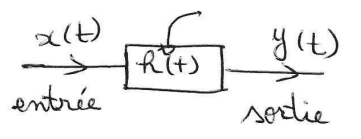
\includegraphics[width = \linewidth]{pic/LTI.png}
                    \end{minipage}
               \end{center}
                \underline{Lineaire} $\implies ax_1(t) + bx_2(t)\overset{\lagrange}{\rightleftarrows}ay_1(t) + by_2(t)$ \\
                \underline{Invariant avex le temp} $\implies \begin{cases}
                    x(t) \implies y(t) \\x(t-t_0) \implies y(t-t_0)
                \end{cases}$ \\
                \underline{Relation} :\begin{itemize}
                    \item $y(t) = h(t)*x(t)$
                    \item $H(s) = \frac{Y(s)}{X(s)}$ ( fonction de transfert)
                \end{itemize}
            \subsection{Circuits electriques}
                \underline{Resistance :}
                \begin{center}
                    \begin{minipage}{0,49\linewidth}
                        domain de temp \\
                        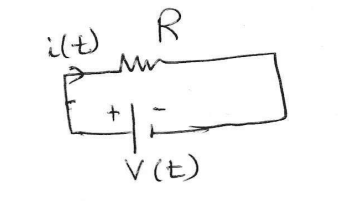
\includegraphics[width=\linewidth]{pic/resistance1.png}
                    \end{minipage}
                    \begin{minipage}{0,49\linewidth}
                        domain de laplace \\
                        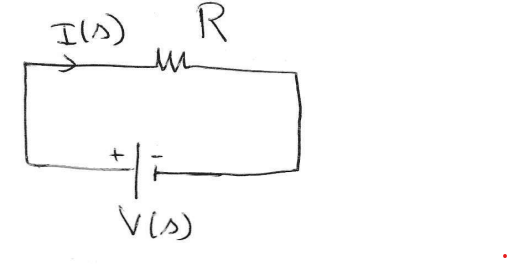
\includegraphics[width=\linewidth]{pic/resistance2.png}
                    \end{minipage}
                    $$ v(t) = Ri(t) \overset{\lagrange}{\rightleftarrows}V(s)=RI(s) $$
                \end{center} 
                \pagebreak
                \underline{Bobine :}
                \begin{center}
                    \begin{minipage}{0,49\linewidth}
                        domain de temp \\
                        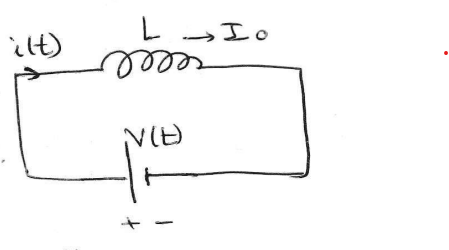
\includegraphics[width=\linewidth]{pic/bobine1.png}
                    \end{minipage}
                    \begin{minipage}{0,49\linewidth}
                        domain de laplace \\
                        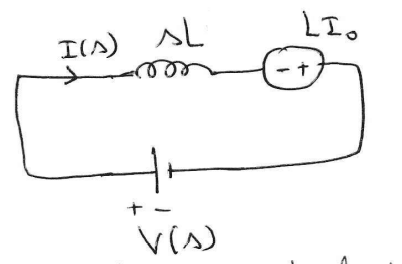
\includegraphics[width=\linewidth]{pic/bobine2.png}
                    \end{minipage}
                    $$ v(t) = L\frac{di(t)}{dt} \overset{\lagrange}{\rightleftarrows}V(s)=L[sI(s) - I_0] $$ 
                    avec $I_0$ est lenergie initiale emagazine
                \end{center} 
                \underline{Condensateur :}
                \begin{center}
                    \begin{minipage}{0,49\linewidth}
                        domain de temp \\
                        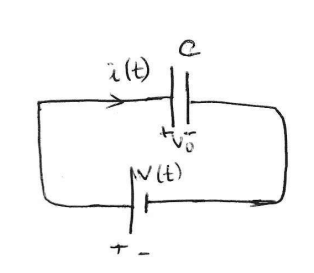
\includegraphics[width=\linewidth]{pic/condonsateur1.png}
                    \end{minipage}
                    \begin{minipage}{0,49\linewidth}
                        domain de laplace \\
                        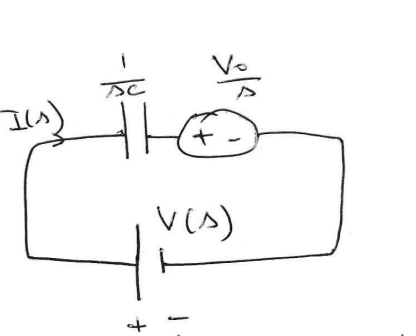
\includegraphics[width=\linewidth]{pic/condonsateur2.png}
                    \end{minipage}
                    $$ i(t)=C\frac{dv(t)}{dt} \overset{\lagrange}{\rightleftarrows}I(s) = C[sV(s)] -CV_0 $$ 
                    $$ V(s) = \frac{I(s)}{sC}+\frac{V_0}{s} $$
                \end{center} 
    \chapter{Series et transformation de fourier}
        \subsection*{Fonctoin periodique}
            Soit $f(t)$ est dite periodique si elle est definie pour toutes les valeur de $t$
                et si elle possede une nombre positif $T$ avex $f(t) = f(t+T)\; , T $periode de $f(t)$
                si $T$ est la plus petit periode , elle est nomme la periode fondamentale de $f(t)$
            \subsubsection*{propriete}
                \begin{itemize}
                    \item si $T$ periode fondamental de $f(t)$ $\implies f(t) = f(t+nT) \; , \; n$: entier
                    \item si $f(t)$ et $g(t)$ ont une periode $T$ ,et $h(t) = af(t)+bg(t)$ avec $ a $ et $b$ sont des $cte$ ,alors $h(t)$ a la meme periode 
                    \item fonction paires : on appelle une fonction $f$ pair si $f(t) = f(-t)$
                    \item fonction impaires : on apelle un fonction $f$ impaire si $-f(t) = f(-t)$
                \end{itemize}
        \section{Serie trigonometrique de Fourier }
            Une fonctoin periodique $f(t)$ avec une periode fondamentale $T$ , develope en serie trigonometrique comme suit : 
            \boxed{f(t) = a_0 +\sum^\infty_{n=1}(a_n\cos(\frac{2\pi}{T}nt)+b_n\sin(\frac{2\pi}{T}nt))} \\ 
            $a_0 , a_n $et $b_n$ sont nommes les coefficient de fourier
            \begin{itemize}
                \item En General
                    \begin{itemize}
                        \item $a_0 = \frac{1}{T}\int^{\frac{T}{2}}_{\frac{-T}{2}}f(t)dt$
                        \item $a_n = \frac{2}{T}\int^{T}_{0}f(t)\cos \left( \frac{2\pi}{T}nt \right) dt$
                        \item $b_n = \frac{2}{T}\int^{T}_{0}f(t)\sin \left( \frac{2\pi}{T}nt \right) dt$
                    \end{itemize}
                \item si $f(t)$ est pair
                    \begin{itemize}
                        \item $a_0 = \frac{2}{T}\int^{\frac{T}{2}}_{0}f(t)dt$
                        \item $a_n = \frac{4}{T}\int^{\frac{T}{2}}_{0}f(t)\cos \left( \frac{2\pi}{T}nt \right) dt$
                        \item $b_n = 0$
                        \item $f(t) = a_0 +\sum^\infty_{n=1}(a_n\cos(\frac{2\pi}{T}nt))$
                    \end{itemize}
                \item si $f(t)$ est inpair
                    \begin{itemize}
                        \item $a_0 = 0$
                        \item $a_n = 0$
                        \item $b_n = \frac{t}{T}\int^{\frac{T}{2}}_{0}f(t)\sin \left( \frac{2\pi}{T}nt \right) dt$
                        \item $f(t) = a_0 +\sum^\infty_{n=1}(b_n\sin(\frac{2\pi}{T}nt))$
                    \end{itemize}
            \end{itemize}
            \underline{Note :}si $T$ est periode fondamental de $f(T)$ \begin{itemize}
                \item $f = \frac{1}{T}$ est frequence fondamental en ($Hz$) hertz
                \item $w = 2\pi f =\frac{2\pi}{T}$ est vitesse angulair en ($\frac{rd}{s}$) radiant par second
            \end{itemize}
            \subsection{Serie de Fourier sous form complexe}
                \begin{itemize}
                    \item $f(t) = C_0 + \sum^\infty_{n=1} 2|C_n| \cos(nw_0t + \theta_n)$
                    \item $C_0 = \frac{1}{T_0}\int_0^{T_0}f(t)dt$
                    \item $C_n = \frac{1}{T_0}\int_0^{T_0}f(t)e^{-inw_0t}dt$
                \end{itemize}
                Relation avec la serie reel : $C_0 = a_0$ et $C_n=\frac{a_n-ib_n}{2}$
        \section{Integral de Fourier}
            Une fonction peut etre represente par un integral appelle integral de fourier \\ \boxed{f(t) = \int^\infty_0 [A(w)\cos(wt) +B(w)\sin(wt)]dw } 
            \begin{itemize}
                \item General 
                    \begin{itemize}
                        \item $A(w) = \frac{1}{\pi}\int^{+\infty}_{-\infty}f(t)\cos(wt)dt$
                        \item $B(w) = \frac{1}{\pi}\int^{+\infty}_{-\infty}f(t)\sin(wt)dt$
                    \end{itemize}
                \item si $f(t)$ est pair   
                    \begin{itemize}
                        \item $A(w) = \frac{2}{\pi}\int^{+\infty}_{0}f(t)\cos(wt)dt$
                        \item $B(w) = 0$
                        \item $f(t) = \int^\infty_0 [A(w)\cos(wt) ]dw$
                    \end{itemize}
                \item si $f(t)$ est impair    
                    \begin{itemize}
                        \item $A(w) = 0$
                        \item $B(w) = \frac{2}{\pi}\int^{+\infty}_{0}f(t)\sin(wt)dt$
                        \item $f(t) = \int^\infty_0 [B(w)\sin(wt)]dw$
                    \end{itemize}
            \end{itemize}
        \section{Transformees de Fourier}
            \subsection{Transforme cosinus de fourier }
                Transforme cosinus de fourier de la fonction pair $f(t)$
                $$ F_c(w) = \sqrt{\frac{2}{\pi}}\int^\infty_0 f(t)\cos(wt)dt $$ 
                Transforme Inverse de cosinus de fourier
                $$ f(t) = \sqrt{\frac{2}{\pi}}\int^\infty_0F_c(w) \cos(wt)dw $$
            \subsection{Transforme sinus de fourier }
                Transforme sinus de fourier de la fonction pair $f(t)$
                $$ F_c(w) = \sqrt{\frac{2}{\pi}}\int^\infty_0 f(t)\sin(wt)dt $$ 
                Transforme Inverse de sinus de fourier
                $$ f(t) = \sqrt{\frac{2}{\pi}}\int^\infty_0F_c(w) \sin(wt)dw $$
            \subsection{Propriete de transforme cosinus et sinus de Fourier}
                \begin{itemize}
                    \item \underline{Linearite} : $F_{c/s}(af(t) + bg(t)) = aF_{c/s}(w)+bG_{c/s}$
                    \item \underline{derive} :\begin{itemize}
                        \item $F_c\{ f^{'}(t) \} = wF_s(w)-\sqrt{\frac{2}{\pi}}f(0)$
                        \item $F_c\{ f^{''}(t) \} = -w^2F_s(w)-\sqrt{\frac{2}{\pi}}f^{'}(0)$
                        \item $F_s\{ f^{'}(t) \} = wF_c(w)$
                        \item $F_s\{ f^{''}(t) \} = -w^2F_s(w)+\sqrt{\frac{2}{\pi}}wf^{'}(0)$
                    \end{itemize}
                \end{itemize}
            \subsection{Transformee de Fourier }
                la transformee de fourier est une technique mathematique utilisee pour transformer une fonction du domain temps ($t,s$) au domai frequence angulair ($w,rd/s$) ou de domain position ($ x,m $)au  domain frequence spatiale ($\beta , rd/m$)
                \\ la transformation : \boxed{\fourier\{f(t)\} =F(w)= \int^{+\infty}_{-\infty}f(t)e^{-iwt}dt }
                \\ la transformation inverse : \boxed{\fourier^{-1}\{ F(w) \} = f(t)= \frac{1}{2\pi}\int^{+\infty}_{-\infty}F(w)e^{iwt}dw }
            \subsection{Propriete de Transfome de Fourier}
                \begin{itemize}
                    \item \underline{Linearite} $\fourier\{ af_1(t) +bf_2(t) \} = aF_1(w) + bF_2(w)$
                    \item \underline{Echelle de temp} $f(at)\overset{\fourier}{\rightleftarrows}\frac{1}{|a|}F(\frac{w}{a})$
                    \item \underline{Decalage} $f(t+t_0)\overset{\fourier}{\rightleftarrows}F(w_0)e^{iwt_0}$
                    \item \underline{Transformation de temp} $f(at-t_0)\overset{\fourier}{\rightleftarrows}\frac{1}{|a|}F(\frac{w}{a})e^{it_0\frac{w}{a}}$
                    \item \underline{dualite} $f(t)\overset{\fourier}{\rightleftarrows}F(w) \implies F(t)\overset{\fourier}{\rightleftarrows} 2\pi f(-w)$
                    \item \underline{Convolution} $\begin{cases}
                        y(t)=x(t)*h(t) \implies Y(w)=X(w).H(w) \\
                        \fourier\{ f_1(t)f_2(t) \} = \frac{1}{2\pi}F_1(w)*F_2(w)
                        \end{cases}$
                    \item \underline{decalage de frequence} $f(t)e^{\pm iw_0t} \overset{\fourier}{\rightleftarrows} F(w\pm w_0)$
                    \item \underline{derive} $\frac{d^nf}{dt^n}\overset{\fourier}{\rightleftarrows}(iw)^nF(w) \; \; , \; \; -itf(t)\overset{\fourier}{\rightleftarrows}\frac{dF(w)}{dw}$
                    \item \underline{integral} $g(t) = \int^t_{-\infty}f(\varphi)d\varphi \implies G(w) = \frac{F(w)}{iw}+\pi F(0)\delta(w)$ avec $F(0) = \int^{+\infty}_{-\infty}f(t)dt$
                \end{itemize}
            \subsection{fonction rectengulair}
                consideron l implusion rectangulaire rect$\left( \frac{t}{T} \right)$
                \begin{center}
                    \begin{minipage}{0,49\linewidth}
                        $\begin{cases}
                            1 & \frac{-T}{2}<t<\frac{T}{2}\\
                            0 & \text{ailleur}
                        \end{cases}$
                    \end{minipage}
                    \begin{minipage}{0,49\linewidth}
                        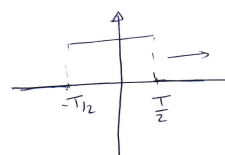
\includegraphics[width = \linewidth]{pic/focntionrectangulair.png}
                    \end{minipage}
                \end{center}
                \underline{Decalage :}
                \begin{center}
                    \begin{minipage}{0,49\linewidth}
                       $g(t) = rect(\frac{t-4}{6})\implies T=6 $ et le centre d implusion a $t=4$
                    \end{minipage}
                    \begin{minipage}{0,49\linewidth}
                        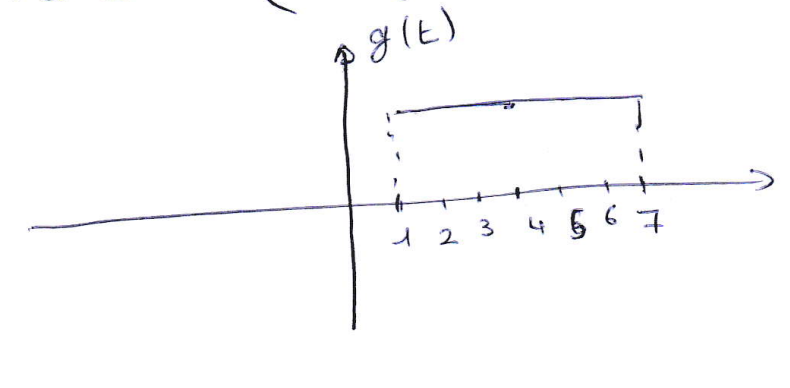
\includegraphics[width = \linewidth]{pic/decalagefonctionrectangulair.png}
                    \end{minipage}
                \end{center}
                \underline{Transforme de fourier de fonction rectangulair}\\
                \boxed{Arect(\frac{t}{T}) \overset{\fourier}{\rightleftarrows}AT \sin_c(\frac{wt}{2}) } avec $\sin_c(x) = \frac{\sin(x)}{x}$(sinus cardinal)
        \section{Theorem de Parseval}
    \chapter{Les polyonme orthogonaux classique}
        \section{Introduction}
            Dans des nombreux problemes physique , on arrive a l'equation differentiell de second ordre , de type hypergeometrique : 
            \begin{center}
                \boxed{\sigma(z)y^{''} + \varphi(z)y^{'} + \lambda y(z) = 0 } (1)
            \end{center}
            avec \begin{itemize}
                \item $\sigma(z)$ : polynome de degre $\leq 2$
                \item $\varphi(z)$ : polynome de degre $\leq 1$
                \item $\lambda(z)$ : $cte$
            \end{itemize}
        \section{Solution polynomial de l'equation hypergeometrique}
            Soit $Y(z)$ est une solution de l equation hypergeometrique , la derive d'ordre $ (n) $ de $ Y(z) $ est aussi une solution de la meme equation  \\
            \underline{Preuve:} \\
            Ona : $ \sigma(z)y^{''}(z) + \varphi(z)y^{'}(z) + \lambda y(z) =0 $\\
            $ \implies$ la Derive : $\sigma^{'}y^{''} + \sigma y^{'''} + \varphi^{'}y^{'}+\varphi y^{''} + \lambda y^{'} =0$ ($ y^{'} = v_1 $ )\\
            $ \implies \sigma v_1^{''} + \varphi_1 v_1^{'} + \mu_1v_1 =0 $ (aussi une equation hypergeometrique)  \\
            avec $ \varphi_1 $ une polynome de premier degre ou moin et d'equation $\varphi_1  = \sigma^{'} + \varphi $ \\
            et $\mu_1 $ est un constant et d'equation  $ \mu_1 =\lambda +\varphi^{'}$ \\
            $ \implies $la Derive second : $\sigma v_2^{''} + \varphi_2v_2^{'}+\mu_2v_2 =0 $ ($ y^{''} = v_2 $ ) \\
            avec $ \varphi_2 $ une polynome de premier degre ou moin et d'equation $\varphi_2  = \sigma^{'} + \varphi_1  = \varphi +2\sigma^{'}$ \\
            et $\mu_2 $ est un constant et d'equation  $ \mu_2 =\lambda_1 +\varphi_1^{'} = \lambda + 2 \varphi^{'} + \sigma^{''}$ \\
            $\implies $ La Deriver d'ordre $(n)$: \boxed{\sigma v_n^{''} + \varphi_nv^{'}_n + \mu_nv_n =0} (2) \\
            avec \begin{itemize}
                \item $ v_n(z)=y^{(n)}(z) $
                \item $ \varphi_n = \varphi + n\sigma^{'} $
                \item $ \mu_n = \lambda + n\varphi^{'} +\frac{n(n-1)}{2}\sigma^{''} $
            \end{itemize}
            Solution particuliere de l'equation hypergeometrique pour $ \mu_n =0 $ \\
            $ \mu_n =0 \implies \sigma v_n^{''} + \varphi_nv_n^{'} =0 $ admet une solution particuliere $ v_n(z) =cte \not = 0 $ \\
            $ \implies \lambda = \lambda_n = - n\varphi^{'} - \frac{n(n-1)}{2}\sigma^{''} $
        \section{Formule de Rodrigues}
            L'equation de rodrigues est une solution de lequation hypergeometrique , elle contien  $ \rho_n(z) $ une fonction caractersiant de l'equation hypergeometrique\\
            $ \left[\sigma(z)y^{''} + \varphi(z)y^{'} + \lambda y(z) = 0\right]\times \rho \implies \sigma(z)y^{''}\rho + \varphi(z)y^{'}\rho + \lambda y(z)\rho = 0$ en peut ecrire cette equation sous la from 
            $(\rho\sigma y^{'})^{'} + \lambda\rho y =0 \implies$ \boxed{(\rho\sigma)^{'} = \rho\varphi} (3) \\
            L equation de rodrigues : \boxed{y_n(z) = \frac{B_n}{\rho(z)}\frac{d^n}{dz^n}\left[\rho(z)\sigma^n(z)\right]} \\
            avec $B_n :$ le constant de normalisation
        \section{Polynomes orthogonaux classiques}
            Formule de Rodrigues de polynomes de Jacobi ,Legendre , Laguerre , Hermite . \\
            Ces polynomes sont  des solution d'equation hypergeometrique 
            \subsection*{Polynome de Jacobi $ P_n^{(\alpha , \beta)} $}
                Ce polynome est la solution de lequation hypergeometrique dans le cas ou 
                \begin{itemize}
                    \item $\sigma = 1-z^2$
                    \item $\varphi = -(\alpha + \beta +2)z +\beta-\alpha$ avec $\alpha$ et $ \beta  $ sont des constant
                \end{itemize} 
                Dans ce cas $\rho$ est d'equation :$ \rho(z) = (1-z)^{\alpha}(1+z)^{\beta} $ \\
                Donc la formule de rodrigues qui est la solution devien : \\
                $ Y_n(z) = P_n^{(\alpha ,\beta)}(z) = B_n(1-z)^{-\alpha}(1+z)^{-\beta}\frac{d^n}{dz^n}\left[ (1-z)^{\alpha + n}(1+z)^{\beta + n} \right] $ \\
                avec $B_n = \frac{(-1)^n}{2^nn!}$\\
                Ona$ \begin{cases}
                    \lambda_n = -n\varphi^{'} - \frac{n(n-1)}{2}\sigma^{''} \\
                    \varphi = -(\alpha + \beta +2)z +\beta-\alpha
                \end{cases} \implies \lambda_n = n(\alpha + \beta + n + 1)$ 
            \subsection*{Polynome de legendre $P_n(z)$}
                Le Polynome de legendre est un cas particuliere de polynome de Jacobi avec $ \alpha = \beta =0 $
                Ce polynome est la solution de lequation hypergeometrique dans le cas ou 
                \begin{itemize}
                    \item $\sigma = 1-z^2$
                    \item $\varphi = -2z$
                \end{itemize} 
                Dans ce cas $\rho$ est constant  \\
                Donc la formule de rodrigues qui est la solution devien : \\
                $ Y_n(z) = P_n(z) =  \frac{B_n}{\rho}\frac{d^n}{dz^n}\left[\rho\sigma^n(z)\right] $ \\
                avec $B_n = \frac{(-1)^n}{2^nn!}$\\
                Ona$ \begin{cases}
                    \lambda_n = -n\varphi^{'} - \frac{n(n-1)}{2}\sigma^{''} \\
                    \varphi = -2z
                \end{cases} \implies \lambda_n = n(n+1)$ 
            \subsection*{Polynome de laguerre $L_n^{(a)}(z)$}
                Ce polynome est la solution de lequation hypergeometrique dans le cas ou 
                \begin{itemize}
                    \item $\sigma = z$
                    \item $\varphi = -z +\alpha +1$ avec $ \alpha > 0 $
                \end{itemize} 
                Dans ce cas $\rho$ est d'equation $\rho = z^\alpha e^{-z}$  \\
                Donc la formule de rodrigues qui est la solution devien : \\
                $ Y_n(z) = L_n(z) =  B_ne^zz^{-\alpha}\frac{d^n}{dz^z}(z^{\alpha + n}e^{-z}) $ \\
                avec $B_n = \frac{1}{n!}$\\
                Ona$ \begin{cases}
                    \lambda_n = -n\varphi^{'} - \frac{n(n-1)}{2}\sigma^{''} \\
                    \varphi  = -z +\alpha +1
                \end{cases} \implies \lambda_n = n$ 
            \subsection*{Polynome d'Hermite $H_n(z)$}
                Ce polynome est la solution de lequation hypergeometrique dans le cas ou 
                \begin{itemize}
                    \item $\sigma = 1$
                    \item $\varphi = -2z$
                \end{itemize} 
                Dans ce cas $\rho$ est d'equation $\rho = e^{-z^2}$  \\
                Donc la formule de rodrigues qui est la solution devien : \\
                $ Y_n(z) = H_n(z) =  \frac{B_n}{e^{-z^2}}\frac{d^n}{dz^n}\left[e^{-z^2}\right] $ \\
                avec $B_n =(-1)^n$\\
                Ona$ \begin{cases}
                    \lambda_n = -n\varphi^{'} - \frac{n(n-1)}{2}\sigma^{''} \\
                    \varphi  = -2z
                \end{cases} \implies \lambda_n = 2n$ 
        \section{Orthogonalite des polynomes de type hypergeometrique}
            $\rho$ verfie la condition $\sigma(z)\rho(z)z^n|_{z=a,b} =0 \implies$ Les polynome de type hypergeometrique seront orthogonaux sur l'intervval (a,b) par rapport a $\rho$ , ces polynome correspondent aux different valeur de $\lambda_n$ \\
            $\implies \int^b_ay_n(z)y_m(z)\rho(z)dz =0$ Si $\lambda_n \not = \lambda_m$
            \subsection*{Polynome de Jacobi}
                $(1-z)^{\alpha +1}(1+z)^{\beta +1}z^k|^b_a =0$ Cette equation est verifier pour $a=-1 $ et $ b=1 $ \\
                Alors le domain est $ (a,b) = [-1,1] $ 
            \subsection*{Polynome de Legendre}
                meme que polyne de jacobi, le domain est $ (a,b) = [-1,1] $ 
            \subsection*{Polynome de Laguerre}
                $z.z^\alpha e^{-z}z^k|_a^b =z^(\alpha + k +1)e^{-z}=0$ \\
                Le domain $(a,b) = [0,+\infty[$
            \subsection*{Polynome d'Hermite}
                $e^{-z^2}z^k|_a^b =0$ \\
                Le domain $(a,b) = ]-\infty , +\infty[$



            
            
            



        
            




\end{document}